\documentclass[a4paper,12pt]{article}
\usepackage[UTF8]{ctex}
\usepackage{fontspec}
\setmainfont{Times New Roman}
\usepackage{geometry}
\usepackage{graphicx}
\usepackage{fancyhdr}
\usepackage{titlesec}
\usepackage{color}
\usepackage{hyperref}
\usepackage{cite}
\usepackage{float}
\usepackage{caption}

% 页面设置
\geometry{left=2.5cm,right=2.5cm,top=2.5cm,bottom=2.5cm}

% 页眉页脚
\pagestyle{fancy}
\fancyhf{}
\fancyhead[L]{基于物理信息驱动的自主理疗具身智能架构研究}
\fancyhead[R]{PIEI Research Proposal}
\fancyfoot[C]{\thepage}

% 标题样式
\titleformat{\section}{\large\bfseries\color{blue}}{\thesection}{1em}{}
\titleformat{\subsection}{\normalsize\bfseries}{\thesubsection}{1em}{}

% 链接设置
\hypersetup{
    colorlinks=true,
    linkcolor=blue,
    filecolor=magenta,      
    urlcolor=cyan,
    citecolor=blue,
}

\title{\textbf{\huge 科研项目建议书：基于物理信息驱动的自主理疗具身智能架构研究} \\ \vspace{0.5cm} \Large Project Proposal: Physics-Informed Embodied Intelligence (PIEI) \\ for Autonomous Thermal Therapy}
\author{\Large 刘晓华 \\ \small Roy Liu}
\date{\today}

\begin{document}

\maketitle
\thispagestyle{empty}

\begin{abstract}
本提案旨在解决医疗具身智能在复杂生物组织交互中的物理感知盲区问题。针对中医艾灸与现代热疗中存在的“不可见不可控”痛点，提出一种融合生物热力学机理与深度学习的 \textbf{物理信息具身智能 (Physics-Informed Embodied Intelligence, PIEI)} 架构。通过构建基于物理常识的世界模型，赋予机器人“透视”皮下热场与预判物理后果的能力，建立Sim2Data合成数据闭环，最终实现理疗过程的精准化与智能化。
\end{abstract}

\vspace{1cm}
\begin{figure}[H]
    \centering
    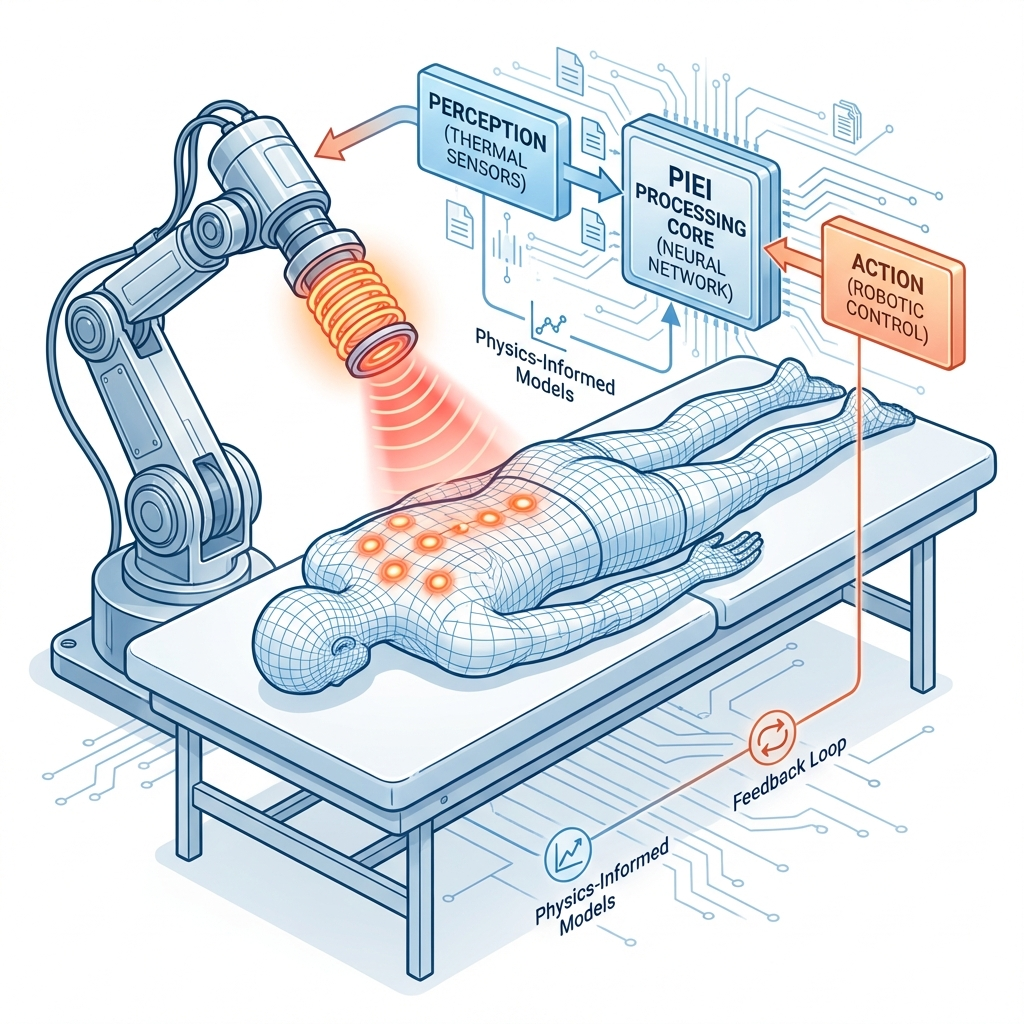
\includegraphics[width=0.95\textwidth]{figs/piei_system_arch_v3.png}
    \caption{PIEI 系统架构图：融合生物热力学世界模型与具身智能感控闭环}
    \label{fig:arch}
\end{figure}

\newpage
\setcounter{page}{1}

\section{一、 WHY：研究背景与立项依据 (Rationale)}

\subsection{1.1 具身智能的“物理缺位”}
当前的具身智能模型（如 RT-2\cite{brohan2023rt}, Mobile ALOHA\cite{zhao2023mobile}, $\pi_0$\cite{pi0_2024}）在几何搬运、语义理解上进展迅速，但在涉及深层物理交互（如热传导、流体力学、生物组织反馈）的精密医疗领域，仍存在“感知浅层、决策盲目”的问题。机器人缺乏对物理后果的预判能力，难以处理不可见的热损伤风险。

\subsection{1.2 医疗理疗的标准化困境}
以艾灸、热疗为代表的非侵入式理疗，极度依赖技师经验，存在三大痛点：
\begin{itemize}
    \item \textbf{不可见性}：皮下热渗透状态无法直观观测，烫伤风险与治疗效果难以平衡。
    \item \textbf{数据饥渴}：真实临床数据（特别是损伤边界数据）因伦理和成本限制极度稀缺\cite{ha2023scaling}。
    \item \textbf{动态干预}：人体呼吸起伏\cite{pavlakos2019expressive}、突发性位移对机械臂的毫秒级闭环补偿提出了极高要求。
\end{itemize}

\subsection{1.3 核心科学问题}
如何构建一个具备生物物理常识的世界模型（Physics-Informed World Model）\cite{karniadakis2021physics}，使其能在仅观测表面的情况下，实现对复杂生物组织内部状态的精准推理与闭环控制？

\section{二、 WHAT：研究目标与预期成果 (Objectives)}

\subsection{2.1 研究目标}
构建一个通用的生物热力学具身智能大脑。该大脑不依赖于特定病种，而是掌握“能量与生物组织交互”的底层物理规律\cite{pennes1948analysis, raissi2019physics}，能够自主规划并安全执行复杂的理疗动作。

\subsection{2.2 预期成果}
\begin{enumerate}
    \item \textbf{Bio-Thermal World Model (生物热力学世界模型)}：一个能预判未来 10 秒内皮下热分布演化的神经网络。
    \item \textbf{PI-VLA Architecture (物理信息驱动的视觉-语言-动作架构)}：实现从人类自然语言指令（如“针对脊柱区域进行雀啄灸”）到精确物理轨迹的映射。
    \item \textbf{Moxi-Bio-Dataset (合成数据集)}：全球首个带物理真值的理疗交互数据集（包含 100k 组多模态轨迹）。
    \item \textbf{学术论文}：在 ICRA/IROS 或 Nature Machine Intelligence, Scientific Reports 等顶刊/顶会发表 1-2 篇高质量论文。
\end{enumerate}

\section{三、 HOW：技术路线与实施方案 (Methodology)}

\subsection{3.1 物理驱动的 Sim2Data 工厂 (算力分配：CPU)}
利用高性能 CPU 集群构建高增益物理仿真引擎\cite{makoviychuk2021isaac}，解决数据稀缺问题。
\begin{itemize}
    \item \textbf{数字化人体建模}：结合 SMPL-X (参数化外壳) 与 Z-Anatomy (解剖级分层结构)，赋予虚拟人体皮肤、脂肪、肌肉的物理属性（热导率、比热容、灌注率）。
    \item \textbf{PDE 方程解算}：在 CPU 上实时解算 Pennes 生物热方程\cite{pennes1948analysis}，模拟热源在复杂组织中的时空扩散。
    \item \textbf{大规模平行仿真}：自动化生成包含各种 BMI（胖瘦）、姿态、环境扰动的合成数据。
\end{itemize}

\begin{figure}[H]
    \centering
    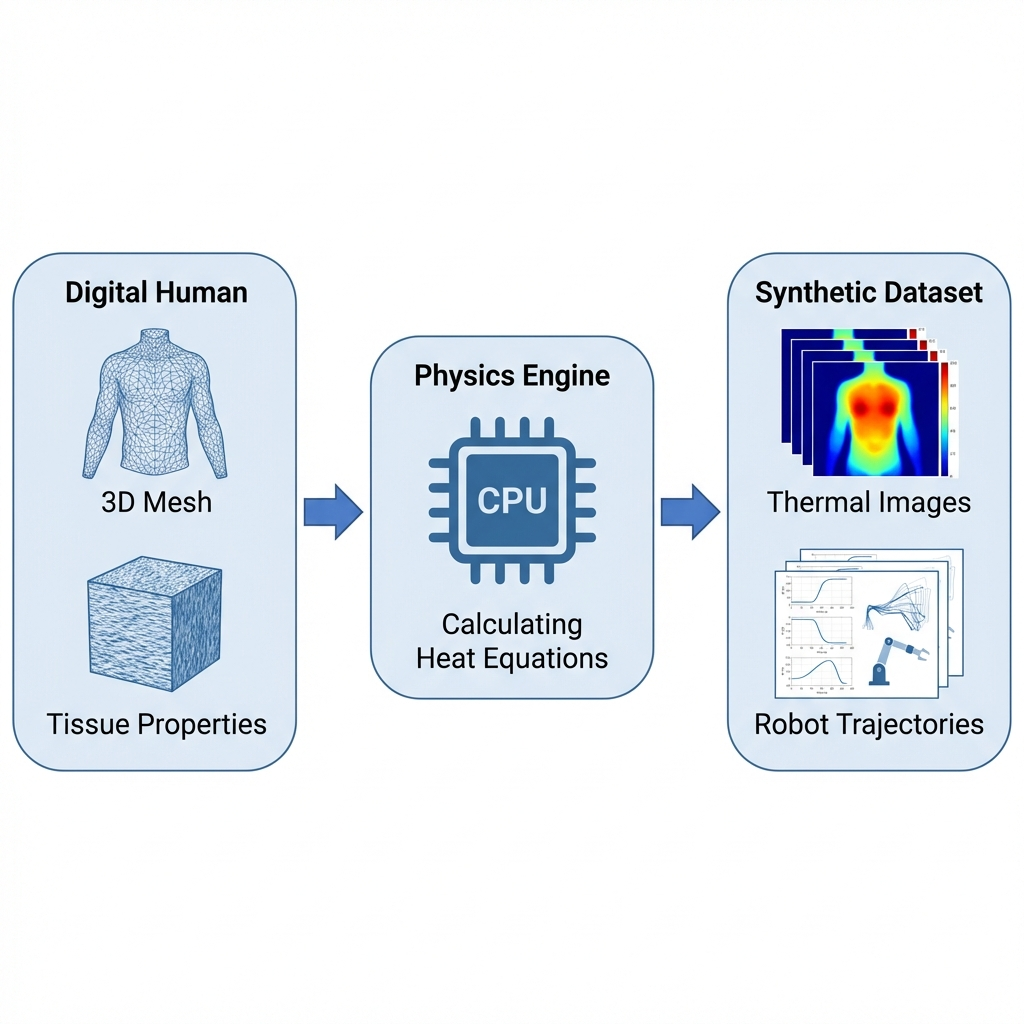
\includegraphics[width=0.9\textwidth]{figs/sim2data_workflow_1769357926569.png}
    \caption{Sim2Data 数据生产流水线：从数字化人体到合成训练数据}
    \label{fig:sim2data}
\end{figure}

\subsection{3.2 跨模态感知与状态观测 (算力分配：L20 GPU)}
利用 L20 GPU 的大显存特性训练深度推理模型：
\begin{itemize}
    \item \textbf{内部状态推理 (Observer)}：利用 Transformer 架构，从表面红外热图序列（Visible）推理出皮下 3D 温度场（Latent）。
    \item \textbf{呼吸与位姿对齐}：通过多模态融合（RGB+Depth），实现对人体微小呼吸运动的实时预测与轨迹补偿\cite{pavlakos2019expressive}。
\end{itemize}

\subsection{3.3 安全约束下的手法策略学习}
\begin{itemize}
    \item \textbf{专家手法参数化}：将中医艾灸的手法（雀啄、回旋等）转化为机器人的微分控制指令。
    \item \textbf{安全性证明 (Control Barrier Functions)}：在执行层嵌入 CBF 算法\cite{ames2019control}，从数学上确保机械臂末端始终处于安全操作包络面内。
\end{itemize}

\subsection{3.4 场景验证（高难度案例验证）}
选取 “癌症术后康复理疗” 作为典型高压场景进行压力测试。
验证逻辑：若模型能处理癌症患者极其敏感、虚弱且高安全标准的理疗需求，则证明其具备泛化至普通康复场景的极强能力。

\section{四、 WITH WHAT：资源配置与工具链 (Resources)}

\subsection{4.1 硬件支撑}
\begin{itemize}
    \item \textbf{NVIDIA L20 GPU (48GB)}：核心推理与视觉渲染引擎，用于运行 NVIDIA Isaac Sim 及大规模 Transformer 模型微调。
    \item \textbf{高性能 CPU 集群}：作为物理计算后端，解算生物热动力学偏微分方程。
    \item \textbf{执行终端}：6 自由度协作机械臂 + 双光谱（可见光+红外）视觉传感器。
\end{itemize}

\subsection{4.2 软件与数据栈 (Open Source Toolchain)}
\begin{itemize}
    \item \textbf{仿真与训练}：NVIDIA Isaac Sim, PyTorch, NVIDIA Warp (GPU 加速物理计算)。
    \item \textbf{解剖模型库}：TotalSegmentator (CT 自动分割), SMPL-X。
    \item \textbf{控制框架}：ROS 2, MoveIt 2。
\end{itemize}

\section{五、 进度规划 (Timeline)}
\begin{itemize}
    \item \textbf{Q1 (环境构建)}：在 CPU 上实现 Pennes 方程解算，在 L20 上搭建虚拟人体理疗实验室。
    \item \textbf{Q2 (数据生产)}：利用 Sim2Data 流程生成 1TB+ 的多模态物理交互数据集。
    \item \textbf{Q3 (模型研发)}：在 L20 上训练热预测网络与 VLA 策略模型。
    \item \textbf{Q4 (验证与产出)}：进行虚实迁移测试，撰写学术论文，并整理开源数据集。
\end{itemize}

\section{项目亮点总结}
\begin{itemize}
    \item \textbf{算力精准匹配}：CPU 负责解算底层物理（Sim），L20 负责感知与推理（AI），资源利用率最大化。
    \item \textbf{学术壁垒高}：避开了纯软件 AI 的红海，通过“物理信息驱动（Physics-Informed）”建立医疗机器人核心壁垒。
    \item \textbf{商业前景广}：技术底座通用，可向下兼容美容、理疗、康复等多个万亿级市场。
\end{itemize}

\bibliographystyle{plain}
\bibliography{refs}

\end{document}
